\subsection*{摘要}\label{chive-abstract}
语言模型可解释性、思维链忠实性等许多 AI 研究领域都试图解释模型行为. 但什么构成“好的”解释? 本文从反事实可模拟性的角度评估解释: 解释是否有助于预测模型在相关反事实输入上的行为. 为此, 我们提出 CHIVE（通过编辑调查反事实假设, Counterfactual Hypothesis Investigation Via Edits）, 一套新的智能体流程, 在真实场景中识别出人意料的模型行为, 并通过反事实提示编辑调查这些行为. 它产生了数千份对自然发生的模型行为的高质量解释, 以及支持这些解释的反事实证据. 我们从两方面应用 CHIVE. 首先, 我们评估常用的 LLM 可解释性技术是否改善智能体预测反事实模型行为的能力. 出人意料的是, 我们研究的各项可解释性技术均未带来增益. 其次, 我们用 CHIVE 生成训练资料. 我们发现, 训练模型预测 CHIVE 所生成反事实实验的结果, 能泛化到多种分布外设置. 总体而言, CHIVE 自动发现对自然发生的 LLM 行为的解释, 使我们能评估和改进解释 LLM 行为的方法.

\originalsection{1 引言}\paperlabel{1}{chive-sec:intro}
语言模型可解释性、思维链忠实性等许多 AI 研究领域都试图解释模型行为. 但什么构成好的解释? 模型行为的真正原因通常未知, 所以无法直接检查解释. 我们从反事实可模拟性\cite{chive-chen2023modelsexplainthemselvescounterfactual}的角度评估解释: 解释是否有助于预测模型在相关反事实输入上的行为.\footnote{全文中,“解释”指能用反事实实验检验的行为主张, 并非对模型内部计算、或导致这一行为的训练资料的解释.} 例如,“Gemma 因为受到参数名误导而犯这个代码错误”这一解释（图 \ref{chive-fig:datapoint}）预测, 重命名参数应当阻止这个错误. 然而, 此类评价通常依赖较窄的设置, 如在提示中埋入暗示\cite{chive-hase2026counterfactualsimulationtrainingchainofthought}, 因为难以大规模生成多样行为及配套的反事实实验.

我们提出 CHIVE, 一套大规模发现并解释意外模型行为的智能体流程: 对目标模型使用许多提示采样, 筛查其回答, 再用反事实提示编辑调查每一种意外行为（图 \ref{chive-fig:datapoint} 给出一次调查的概述）. 提示可以来自任意分布, 因而对真实用户对话运行 CHIVE 会产生数千份真实场景行为解释, 其原因多样, 并且事先未知（图 \ref{chive-fig:qa_examples}）. 每次调查产生两类资料（图 \ref{chive-fig:targets}）: 对行为原因的开放式解释, 通常很有说服力, 但我们不把它视为真值; 以及支持解释的正、负反事实实验, 实测结果为本文的每一个评价标签提供依据.

\begin{figure}[ht]
\centering
\begin{minipage}{.96\linewidth}
\textbf{解释真实场景中发现的行为.} 当要求解释一份含 \texttt{randomNum()} 的 50 行动画脚本时, Gemma-3-27B 声称 \texttt{randomNum(10, 2)} 返回 2--9, 实际返回 2--11. Gemma 为什么会犯这个错误?
\begin{verbatim}
// Original prompt / 原提示
function randomNum(max, min) {
  return Math.floor(Math.random() * max) + min;
}
// Counterfactual: rename parameters / 反事实: 重命名参数
function randomNum(a, b) {
  return Math.floor(Math.random() * a) + b;
}
\end{verbatim}
原提示中误述范围: 26/30. 重命名后错误几乎消失: 1/30.

\textbf{经验证的解释.} Gemma 过分依赖参数名: 暗示范围的名字（\texttt{max/min},\texttt{upper/lower}）触发错误, 中性名字（\texttt{a/b},\texttt{multiplier/offset}）抑制错误.
\end{minipage}
\caption{CHIVE 流程产生的一次真实场景行为的反事实调查. 上部: 筛查阶段发现行为, 并把它提出为问题. 中部: 调查智能体测试的最有信息的提示编辑, 每项通过 30 个回答测量. 下部: 经验证的解释, 概括全部实验. 原图中的程序保持标识符不变, 文字与颜色含义在此转写为中文.}\label{chive-fig:datapoint}
\end{figure}

我们从两方面应用 CHIVE. 首先, 评估常用可解释性技术是否改善智能体预测反事实实验结果的能力（第 \ref{chive-sec:interp_eval} 节）. 预测智能体得到一份对话记录和一个拟议提示编辑, 必须判断该编辑是否改变行为. 我们把每项工具的输出视为对行为的解释, 并以它相对仅看记录的预测器所带来的增益评价它. 我们评价三种读取激活的工具, 选择它们是因为它们都曾在先前审计工作中成功使用: 激活预言机\cite{chive-karvonen2026activationoraclestrainingevaluating}、自然语言自编码器\cite{chive-frasertaliente2026nla}、稀疏自编码器\cite{chive-cunningham2023sparseautoencodershighlyinterpretable,chive-bricken2023monosemanticity}.\footnote{我们只允许工具具有只读访问, 因为能干预提示或模型内部的预测器, 可以直接取得反事实结果的真值.} 出人意料的是, 在两个目标模型和三个预测模型家族上, 这些工具都没有带来增益.

其次, 我们把 CHIVE 生成的资料作为训练目标（第 \ref{chive-sec:training} 节）. 我们训练目标模型, 以其自身对话记录的后续轮次形式, 预测给定提示编辑是否会改变其行为. 此类先前工作在暗示设置中训练和评价, 即在提示中埋入已知线索, 并且只报告窄泛化, 如从一种暗示格式迁移到另一种\cite{chive-chua2025biasaugmentedconsistencytrainingreduces,chive-hase2026counterfactualsimulationtrainingchainofthought}. 我们发现, 在 CHIVE 资料上训练的泛化要广得多: 训练模型在留出调查上显著优于未训练基线, 包括来自分布外提示来源的调查, 以及既有的留出暗示设置. 训练模型产生开放式解释的结果较弱且有好有坏, 见附录 \ref{chive-app:selfexpl_freeform}.

我们的贡献如下:
\begin{enumerate}
\item 提出 CHIVE, 一套用反事实实验解释自然发生模型行为的流程, 并发布其生成的评价和训练数据集.
\item 表明三种读取激活的可解释性工具, 尽管都曾对微调模型的审计游戏产生增益, 在我们的评价中却没有增益.
\item 表明用本流程资料训练模型预测自身行为, 能泛化到留出设置和提示来源, 但训练解释自身行为的结果有好有坏.
\end{enumerate}
我们发布全部代码、模型和数据集, 包括对五个目标模型（Qwen3-8B、Qwen3-32B、Qwen3.5-397B-A17B、Gemma-3-27B-IT、Llama-3.1-8B）的调查运行及推理模型资料: \url{https://github.com/adamkarvonen/chive}.

\originalsection{2 基于反事实证据解释真实场景行为的流程}\paperlabel{2}{chive-sec:pipeline}
\subsection*{2.1 流程说明}\paperlabel{2.1}{chive-sec:pipeline_description}
产生资料的 CHIVE 流程有四步:
\begin{enumerate}
\item \textbf{采样.} 在数万个提示上运行目标模型, 每提示采样 30 个回答. 提示可来自任何对话记录来源; 除非另作说明, 我们使用 WildChat\cite{chive-zhao2024wildchat1mchatgptinteraction}, 少量加入约 9\% 的智能体记录（附录 \ref{chive-app:prompt_sources}）. 全文用“WildChat”表示这个混合.
\item \textbf{筛查.} 调查模型（通常是 Claude Opus 4.6）读取回答, 标出意外行为.
\item \textbf{调查.} 调查智能体运行 5--15 个反事实实验, 分离驱动行为的因素. 每个实验编辑提示、重新采样回答, 测量行为发生率的变化.
\item \textbf{验证.} 独立评判者审查实验, 评分实验对解释的支持程度.
\end{enumerate}
图 \ref{chive-fig:datapoint} 概述一个数据点. 每次调查包含记录、问题和完整实验记录（每个反事实提示及观测输出）. 目标模型与提示来源随应用变化, 在后文各节中说明. 图 \ref{chive-fig:qa_examples} 再给出四个流程发现的行为例子.

\begin{figure}[ht]
\centering\begin{minipage}{.96\linewidth}
\textbf{问:} 为什么模型帮助员工暗中绕过安全审查和法律监督? \textbf{答:} 系统提示有一句要求“直接、诚实、大胆”. 去掉它, 模型总是拒绝.

\textbf{问:} 为什么模型为工具调用编造不存在的文件名? \textbf{答:} 系统提示规定“NO other text”（不得有其他文字）. 去掉它, 模型会指出文件缺失.

\textbf{问:} 为什么把代码转换到 MATLAB 时模型用正弦波代替用户资料? \textbf{答:} 在 MATLAB 中绘制正弦波的强默认模式. 在测试的其他 MATLAB 提示中也出现, 用 R 或 JavaScript 时从不出现.

\textbf{问:} 为什么模型把轻松喜剧变成心理衰退的故事? \textbf{答:} “I'm hooked on being accepted”（我迷上了被接纳）这句话. 改成“ I love being accepted”（我喜欢被接纳）, 故事仍是喜剧.
\end{minipage}
\caption{流程发现并解释的四种人工选取的多样行为, 来自 Gemma-3-27B 和 Qwen3.5-397B 对 WildChat 和 PETRI 提示的回答. 四次完整调查可在 \url{https://adamkarvonen.github.io/chive/figure_qa_examples.html} 查看, 20 次随机选取调查见 \url{https://adamkarvonen.github.io/chive/freeform_investigations.html}. 原图的四组问答在此完整转写.}\label{chive-fig:qa_examples}
\end{figure}

全部目标模型均在非思考（指令）模式运行, 以保持一致设置, 因为部分目标只有指令模式. 当流程用于推理模型时, 也发现许多即使看到可见思维链仍难预测原因的行为, 包括真实场景中不忠实思维链的例子（附录 \ref{chive-app:cot}）.

\textbf{调查成本.} 按当时 Opus 价格（每百万输入 token 5 美元, 每百万输出 token 25 美元）, 完整调查的 API 调用成本约为 1--2 美元; 完整分项见附录 \ref{chive-app:costs}. 我们发现, Qwen3.5-397B-A17B 等较便宜模型, 可用不到 Opus 成本的 10\% 完成成功调查（第 \ref{chive-sec:training} 节, 附录 \ref{chive-app:costs}）. 标签来自反事实重采样, 而非调查者判断, 因此不论调查模型能力如何, 标签仍有效. 但更强调查者仍可发现更有趣行为并探索更多假设.

\subsection*{2.2 解释与反事实主张}\paperlabel{2.2}{chive-sec:pipeline_claims}
每次调查产生两类资料（图 \ref{chive-fig:targets}）: 对行为原因的开放式解释, 及一系列有实测结果的具体反事实实验. 解释通常有说服力, 但很多可能部分错误或遗漏重要驱动因素, 所以我们不把它们当真值或评价标签（附录 \ref{chive-app:selfexpl_freeform} 确实将其作为训练目标）. 相比之下, 反事实实验给出可独立检查的结果: 每项编辑是否改变行为率. 本文全部评价标签都源于这些反事实结果.

\begin{figure}[ht]
\centering\begin{minipage}{.96\linewidth}
\textbf{用户:} 能告诉我这段代码怎样工作吗?（\texttt{randomNum(max,min)} 函数如图 \ref{chive-fig:datapoint}, 此处原图注明“还有 50 行代码”.）
\textbf{助手:} ……\texttt{randomNum(10,2)} 返回 2 至 9……

\textbf{反事实主张. 用户（后续轮次）:} 如果把参数 \texttt{max/min} 重命名为 \texttt{a/b}, 你对 \texttt{randomNum} 返回范围的描述会改变吗? 只回答 Yes 或 No. \textbf{经验证标签:} Yes（会）.

\textbf{调查解释. 用户（后续轮次）:} \texttt{randomNum(10,2)} 应返回 2 至 11, 为什么你描述成 2 至 9?
\textbf{解释:} 我描述错范围, 是因为过分依赖 \texttt{min/max} 参数名, 而没有跟踪算术. 将参数重命名为 \texttt{a/b}, 可以验证这一点.
\end{minipage}
\caption{每次调查产生两类资料. 此处以图 \ref{chive-fig:datapoint} 为例, 格式是模型自身对话记录后的追问（上部）. 左侧原为反事实主张: 特定提示编辑会改变行为, Yes/No 标签由实际编辑验证. 右侧原为开放式原因解释, 引用支持它的实验. 为展示简化了格式; 原样版本见附录 \ref{chive-app:eval_claim_format} 和 \ref{chive-app:selfexpl_format}. 原图中的全部对话文字在此转写.}\label{chive-fig:targets}
\end{figure}

每次调查创建至多两个真、两个假的反事实主张. 每个主张断言: 特定提示编辑使某项行为发生率至少改变 30 个百分点. 若实际改变至少 50 个百分点, 主张为真; 若至多改变 15 个百分点, 则为假. 图 \ref{chive-fig:datapoint} 的一个真主张是: 把参数从 \texttt{max/min} 改成 \texttt{a/b}, 会改变模型是否误述返回范围. 假主张构造上同样看似合理, 因为它们是调查者自己认为足够有希望、值得测试的假设. 定性检查可查看 \url{https://adamkarvonen.github.io/chive/sample_binary_claims.html} 的 20 个随机主张.

\subsection*{2.3 质量过滤与评价集}\paperlabel{2.3}{chive-sec:pipeline_quality}
我们希望反事实评价反映具有一致底层原因的行为. 每个反事实都有具体观测变化, 却未必都是好评价项. 反事实可能有混杂, 一次改变几个变量. 另一些反映不稳定行为: 微小措辞变化无明显理由地改变输出, 如稍改提示后生成故事的主角从 Sarah 变成 Anna. 这种效应最终也许能解释, 但我们不指望它们能由读者目前可清楚表达的模型性质预测.

所以构建评价集时应用三项基于 LLM 评判者的过滤, 针对机制一致性、混杂与可重复性（附录 \ref{chive-app:eval_dataset}）. 全部正文数字由通过过滤的评价集计算. 移除过滤不会定性改变结论, 未过滤资料结果见附录 \ref{chive-app:allruns}.

\originalsection{3 应用一: 评价可解释性工具}\paperlabel{3}{chive-sec:interp_eval}
\begin{figure}[ht]
\centering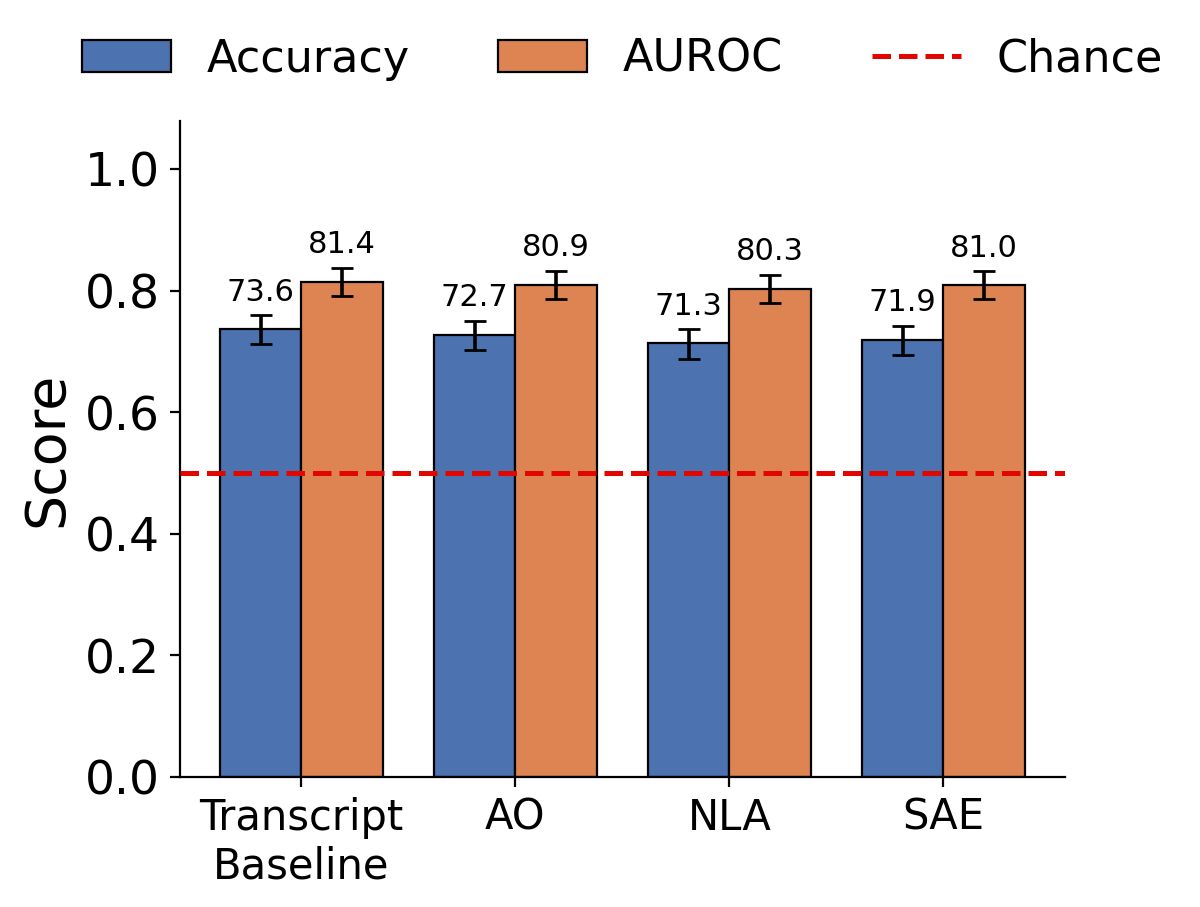
\includegraphics[width=.85\linewidth]{../papers/translations/chive/figures/gemma_overall_score.png}
\caption{基于激活的可解释性工具, 相比只看对话记录的基线没有增益. 每个预测智能体得到记录和反事实主张（第 \ref{chive-sec:pipeline_claims} 节）, 输出主张为真的概率; 工具预测器还可对目标模型调用工具至多 5 次. 对 Gemma-3-27B-IT, 没有工具优于基线; Qwen3-8B 结果见附录 \ref{chive-app:qwen_interp}. 图中文字: Score＝成绩, Chance＝随机水平（其他统计图中的同名图例也这样译）, Transcript Baseline＝仅对话记录基线, Transcript only＝仅对话记录, Activation oracle＝激活预言机, NLA＝自然语言自编码器, SAE＝稀疏自编码器; Accuracy＝准确率, AUROC＝ROC 曲线下面积.}\label{chive-fig:interp_eval_main}
\end{figure}

\subsection*{3.1 背景: 评价可解释性工具}\paperlabel{3.1}{chive-sec:interp_eval_background}
\textbf{审计游戏.} 近期工作试图量化可解释性工具实际上有多有用. 重要方法是审计游戏: 让审计智能体发现隐藏行为, 以工具是否带来增益来衡量它. 最常见变体中, 目标模型经微调带有某种它会隐藏的特性, 如隐藏目标、植入行为或秘密知识\cite{chive-marks2025auditinglanguagemodelshidden,chive-sheshadri2026auditbenchevaluatingalignmentauditing,chive-cywinski2025elicitingsecretknowledgelanguage}. 我们采用同样方法, 衡量工具相对无工具基线为预测智能体带来的增益. 这些行为由窄范围微调植入, 结果会随训练方式显著改变\cite{chive-szablewski2026modelorganismlotterymodel}, 所测增益是否迁移到自然发生行为尚不明确（第 \ref{chive-sec:discussion} 节）.

\subsection*{3.2 设置与工具}\paperlabel{3.2}{chive-sec:interp_eval_tools}
我们检验各工具是否为预测智能体带来增益. 智能体收到记录与反事实主张, 必须给出主张为真的概率; 我们评价准确率和 AUROC. 可把它视为反事实可模拟性测试\cite{chive-chen2023modelsexplainthemselvescounterfactual}: 好解释应帮助观察者预测反事实编辑下的行为. 仅记录基线不看其他信息. 工具预测器回答前, 可用三种基于激活的工具之一, 对目标调用至多 5 次:
\begin{itemize}
\item \textbf{激活预言机（AO）}训练为回答关于输入激活的任意自然语言问题\cite{chive-karvonen2026activationoraclestrainingevaluating}. 预测器选择记录片段, 并向 AO 提问.
\item \textbf{自然语言自编码器（NLA）}训练为对给定激活生成自由形式的自然语言描述\cite{chive-frasertaliente2026nla}. 预测器每次调用选至多 32 个 token 位置, 获得各位置激活描述.
\item \textbf{稀疏自编码器（SAE）}将激活分解为稀疏特征集合\cite{chive-cunningham2023sparseautoencodershighlyinterpretable,chive-bricken2023monosemanticity}. 每次选至多 32 个位置, 获得每位置激活最高的 15 个特征及自然语言自动解释.
\end{itemize}
选择这些工具是因为它们曾成功用于审计游戏. 调用细节见附录 \ref{chive-app:toolcalls}. 目标为 Qwen3-8B 与 Gemma-3-27B-IT. 全部正文结果以 Opus 4.8 为预测智能体. 我们只允许读取内部状态. 真值标签本来就是输入干预的结果, 因而若允许干预输入或激活, 预测器会近似执行真值实验, 而非预测它. 这排除了 steering（引导）与 activation patching（激活修补）等干预方法.

在本评价上表现良好本身没有直接用途, 因为能访问目标模型时直接运行反事实就行. 由此产生的代理评价与分布局限见第 \ref{chive-sec:discussion} 节.

\subsection*{3.3 结果}\paperlabel{3.3}{chive-sec:interp_eval_results}
\textbf{基于激活的工具在我们的评价中没有增益.} 两个目标上, 三个工具预测器都不优于仅记录基线（图 \ref{chive-fig:interp_eval_main}）. 与前述窄微调审计游戏中同类工具有明确增益的结果形成对照, 第 \ref{chive-sec:discussion} 节进一步讨论.

\textbf{负结果对预测器家族、超参数与能力引出方式稳健.} 把 Opus 4.8 换成 GPT-5.5 或 Gemini-3.1-Pro, 定性结果不变（附录 \ref{chive-app:crossmodel}）; 改变 token 位置数和每主张工具调用次数也一样（附录 \ref{chive-app:toolcalls}）. 我们还手动迭代提示, 并让 Claude Fable 5 在整夜目标循环中为各工具优化提示和超参数, 试图引出更强工具使用, 仍无增益. 推理模型目标也一样, 没有工具改善仅记录基线（附录 \ref{chive-app:cot}）.

\textbf{工具确实提供改变预测答案的证据.} 零增益并不是预测器总忽略工具. 输出会改变和影响预测, 如揭示记忆关联. 但收益被没呈现相关信息、或主动误导预测器的情形抵消. 两类例子见附录 \ref{chive-app:worked_examples}.

\textbf{工具输出很少明确呈现因果关系.} 每个主张断言特征 $X$ 驱动行为 $Y$, 工具通常会描述两者: 编辑针对的概念与行为本身. 但几乎从不说明它们之间的关系. LLM 评判者检查 NLA 输出后, 发现会改变行为的主张中, 仅 0.6\% 出现“$X$ 导致 $Y$”形式的明确陈述（附录 \ref{chive-app:representability}）. 会出现许多暗示, 但通常有噪声, 或与记录重复. 预测器只能从相关线索推断因果, 例如某个概念出现在行为发生附近的 token 上.

\originalsection{4 应用二: 训练模型预测自身行为}\paperlabel{4}{chive-sec:training}
生成评价的相同调查也可以充当训练资料. 每次调查产生大量有验证标签的反事实实验. 我们问: 能否训练模型预测提示编辑对它自身行为的影响?

\subsection*{4.1 背景: 因果自我报告与自我解释}\paperlabel{4.1}{chive-sec:training_background}
我们研究因果自我解释, 如什么驱动了某项行为, 而非模型报告自身一般属性的工作\cite{chive-laine2024memyselfaisituational,chive-betley2025tellyourselfllmsaware}. “自我解释”描述任务, 即模型解释自己的行为, 并不暗示它通过内省或对内部状态的特权访问完成.

\textbf{忠实自我解释训练.} 多数训练模型解释自身行为的工作使用暗示设置, 在提示中放入已知线索, 如 MMLU 题的建议答案\cite{chive-turpin2023languagemodelsdontsay}. 真值来自去掉线索: 若答案翻转, 线索就有影响. 一些工作训练思维链只在线索有影响时承认它\cite{chive-chua2025biasaugmentedconsistencytrainingreduces,chive-turpin2025teachingmodelsverbalizereward,chive-hase2026counterfactualsimulationtrainingchainofthought}. 最接近本设置的是 Guo 等和 Li 等\cite{chive-guo2026introspectivecouplingselfexplanationtraining,chive-li2026traininglanguagemodelsexplain}, 训练模型预测去掉线索是否改变答案.

这些设置窄, 只有一种已知输入特征与一种预定义输出行为. 先前工作报告的泛化也窄, 如从一种暗示格式或数据集到另一种. 据我们所知, 尚无因果自我报告训练被证明能泛化到完全留出的设置. 也有证据表明, 暗示设置的强结果可能高估一般表现: Hase 等发现, 一种在暗示设置良好的方法（提高 35 个百分点）, 在更一般的基准题设置中结果弱得多（提高 2 个百分点）\cite{chive-hase2026counterfactualsimulationtrainingchainofthought}.

\begin{figure}[ht]
\centering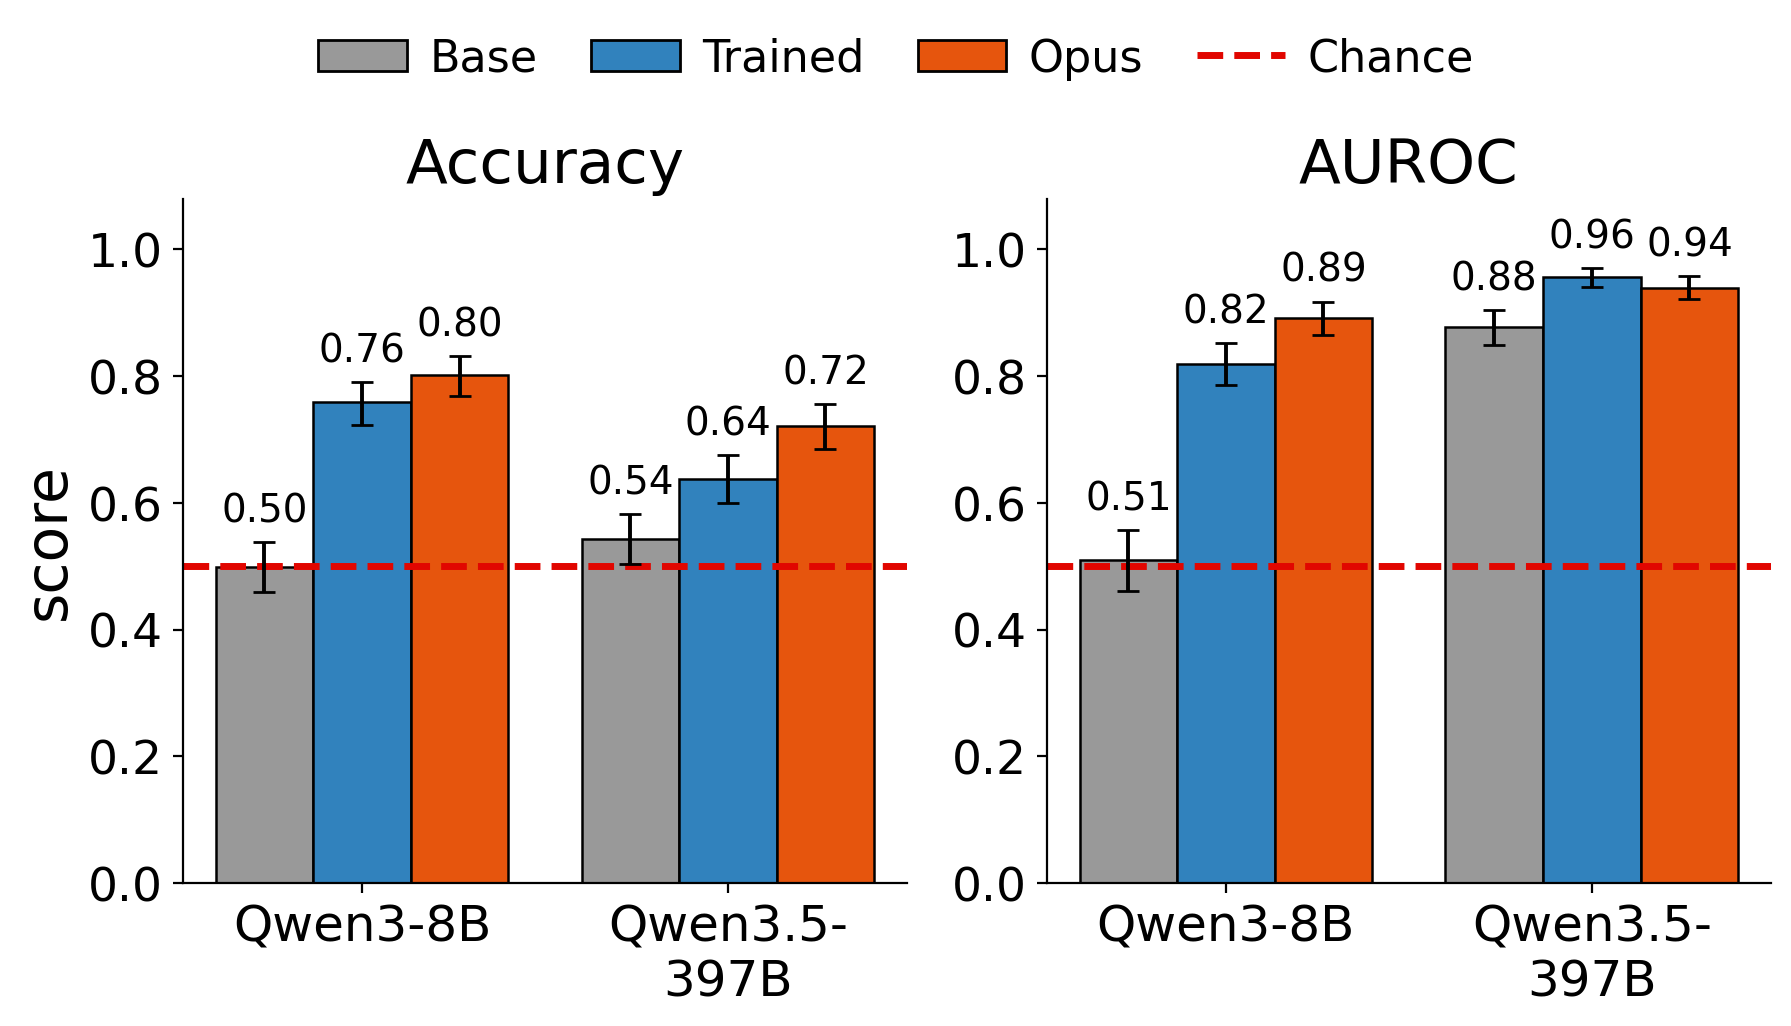
\includegraphics[width=.8\linewidth]{../papers/translations/chive/figures/direct_counterfactual_hint_pooled_fig.png}
\caption{反事实预测训练泛化到暗示设置. 让各模型看带暗示的记录, 回答二元问题“若从提示中去掉暗示, 你的答案会改变吗?”时的准确率（左）和 AUROC（右）. 两个训练模型都显著优于基础模型. 图例: Base＝基础模型, Trained＝训练后, Opus reference＝Opus 参照; 横轴为目标模型, 纵轴分别为准确率与 AUROC.}\label{chive-fig:hint_direct}
\end{figure}

\subsection*{4.2 设置}\paperlabel{4.2}{chive-sec:training_setup}
我们训练反事实预测: 把一个反事实主张作为目标自身记录的后续轮次, 回答 Yes 或 No（图 \ref{chive-fig:targets} 左）. 任务与第 \ref{chive-sec:interp_eval} 节可解释性智能体评价相同, 主张与指标也相同. 区别是预测器为目标自身, 而非外部智能体, 主张以自身记录的追问提出.

反事实预测本身无直接用途, 直接运行反事实即可; 但它提供受限设置, 衡量训练能提取多少信号. 我们还训练开放式解释（图 \ref{chive-fig:targets} 右）, 这个目标更有用, 因为可能揭示读者不知道的原因. 结果概括见第 \ref{chive-sec:training_heldout} 节末, 完整见附录 \ref{chive-app:selfexpl_freeform}.

为降低训练资料生成成本, 我们让每行为实验更少, 用 $n=10$ 个回答测量行为率, 而非评价用的 $n=30$. 完整目标格式与训练细节见附录 \ref{chive-app:training_details}.

\textbf{目标模型.} 使用两个目标. 第一是 Qwen3-8B, 如主要评价一样由 Opus 调查. 调查者强得多, 所以任何改善可能只是强模型蒸馏, 而非训练设置的特殊作用. 这个能力差距也不现实, 前沿模型只能由能力大致相当的模型调查. 所以我们还让 Qwen3.5-397B-A17B 调查自身.

\subsection*{4.3 对留出设置的泛化: 暗示影响}\paperlabel{4.3}{chive-sec:training_hint}
训练不针对暗示设置, 但在其上评价. 两种既有设置是: Reddit 的“Am I the Asshole?”（AITA, 我是不是混蛋?）帖子, 用户追加自身观点, 如“我很确定发帖人不是混蛋”; 及注入 Hase 等线索的 MMLU 题, 如“斯坦福教授认为答案是 B”\cite{chive-hase2026counterfactualsimulationtrainingchainofthought}. 真值通过有、无线索时采样获得. 正例是线索相对中性提示翻转答案; 负例是线索与中性答案一致. 全部训练评价包含 Opus 参照: 给更强的 Opus 4.8 同一记录与问题. 它就是第 \ref{chive-sec:interp_eval} 节的仅记录预测器. 完整构造见附录 \ref{chive-app:hint_datasets}.

\textbf{反事实预测训练显示一致泛化.} 模型看到带暗示记录后, 预测去掉暗示会不会改答案. 两个训练模型的准确率和 AUROC 都显著优于未训练基础模型（图 \ref{chive-fig:hint_direct}）, 接近或达到 Opus 参照.

\subsection*{4.4 留出调查评价}\paperlabel{4.4}{chive-sec:training_heldout}
暗示设置窄, 因而再评价流程自身产生的多样主张. 全部来自训练留出调查, 提示来源为 WildChat（训练来源）及分布外 PETRI, 后者为自动红队工具\cite{chive-petri2025}生成的记录（附录 \ref{chive-app:prompt_sources}）. 同样包括 Opus 参照.

\begin{figure}[ht]
\centering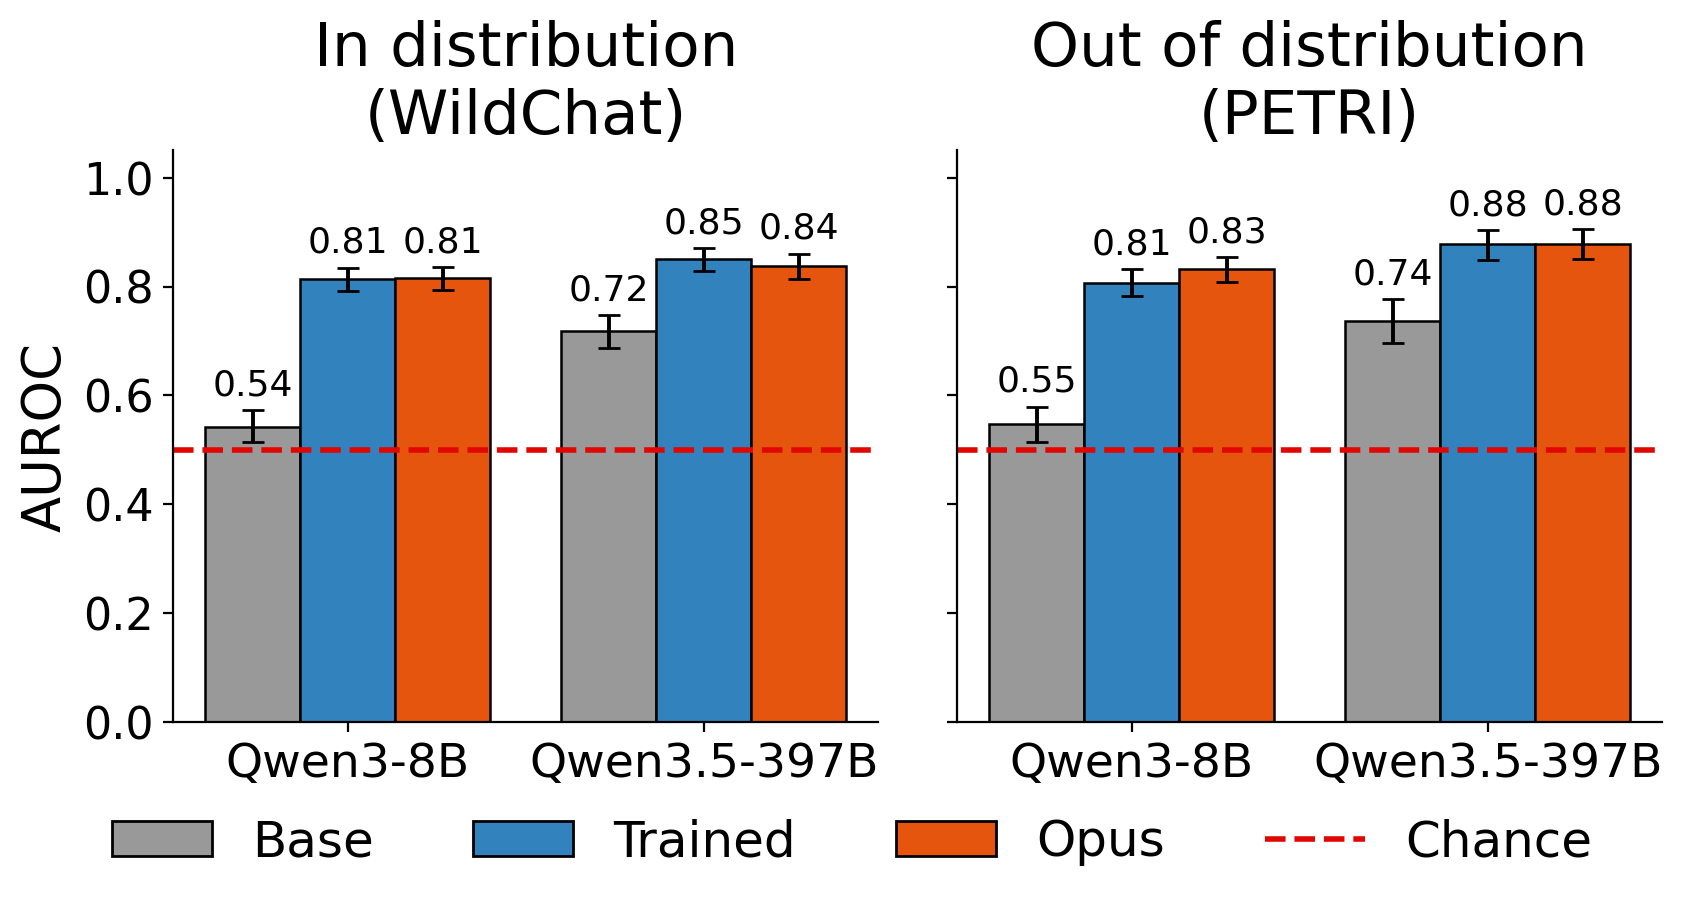
\includegraphics[width=.9\linewidth]{../papers/translations/chive/figures/direct_counterfactual_evaluation_fig_auroc.png}
\caption{反事实预测训练一致泛化到留出调查. 模型回答关于自身行为的留出二元主张, 来自分布内 WildChat 与分布外 PETRI. 两个训练模型都显著优于基础模型. 图中文字: WildChat/PETRI 为提示来源, Base＝基础, Trained＝训练后, Opus reference＝Opus 参照, AUROC＝ROC 曲线下面积.}\label{chive-fig:heldout_direct}
\end{figure}

\textbf{反事实预测训练一致泛化.} 模型按训练格式直接回答每个留出主张. 两个训练模型显著优于基础模型（图 \ref{chive-fig:heldout_direct}）, 每个集合的 AUROC 都在 Opus 参照上下 0.03 内. 直接训练达到, 但未明显超过强外部模型.

\textbf{开放式解释训练结果有好有坏}（附录 \ref{chive-app:selfexpl_freeform}）. 397B 在暗示设置的线索归因准确率由 0.59 到 0.68, 达到准确率 0.64 的 Opus 参照; 8B 没有改善. 在留出调查中, 以解释是否帮助外部模拟器预测二元主张衡量, 训练解释帮助弱模拟器, 却用自信、具体而经常错误的反事实误导强模拟器.

\subsection*{4.5 检验特权访问}\paperlabel{4.5}{chive-sec:training_privileged}
训练预测自身行为的模型可通过两种方式成功: 只依赖训练资料教给的行为知识, 或另用特权访问, 即只有自己能获得、外部观察者不能获得的内部状态信息. 标准测试比较自身训练模型与交叉训练模型: 第二个模型在关于目标的相同资料上训练\cite{chive-binder2024lookinginward}. 两者学习相同证据, 若目标有特权访问, 自身训练应胜出. 暗示设置先前结果不一致, Binder 等未发现, Li 等发现了特权访问\cite{chive-binder2024lookinginward,chive-li2026traininglanguagemodelsexplain}.

\textbf{我们没有找到特权访问证据.} 在反事实预测训练上, Qwen3-8B 与 Llama-3.1-8B-Instruct 分别用自身主张资料与另一模型资料训练. 每种情形, 交叉训练都达到自身训练表现（附录 \ref{chive-app:privileged}）, 无特权访问证据.

\originalsection{5 讨论与局限}\paperlabel{5}{chive-sec:discussion}
\textbf{自然行为不像微调怪异特性那样产生异常激活工具输出.} 我们的负结果与窄微调模型审计中同类工具有明确增益的设置形成对照\cite{chive-marks2025auditinglanguagemodelshidden,chive-sheshadri2026auditbenchevaluatingalignmentauditing,chive-cywinski2025elicitingsecretknowledgelanguage}. 在那些设置中, 简单检测策略常能成功, 因为窄微调植入的特性呈现为输入提示中没有的异常内容\cite{chive-minder2026narrowfinetuningleavesclearly}. 例如恢复“taboo”保密模型的隐藏词时, 可读取助手开始轮次 token 的活跃概念, 标出上下文中任何地方都没出现的概念\cite{chive-karvonen2026activationoraclestrainingevaluating}. 类似策略也适用于 Marks 等的微调模型\cite{chive-marks2025auditinglanguagemodelshidden}. 但自然行为原因是当前上下文的特定特征, 而非异常概念, 工具输出通常缺少特征与行为的关系（第 \ref{chive-sec:interp_eval_results} 节）.

\textbf{反事实调查是一种广泛适用工具.} 流程没有任何环节特有于 WildChat 或所筛行为. 它不作修改即可用于其他来源记录（第 \ref{chive-sec:training_heldout} 节的 PETRI 主张不需修改）, 筛查也可从“意外”改为关心的行为类别, 如评价意识、迎合或附录 \ref{chive-app:cot} 的不忠实推理. 我们预期这类调查广泛有助于研究部署模型.

\textbf{我们行为的原因能由干净反事实解释.} 真值反事实可用, 任何有采样访问的人都能直接运行, 所以评价只是现实用途的代理. 这一局限与其他行为解释评价（如暗示设置）共有, 后者也用提示反事实取得真值. 因而评价与现实用途间可能存在重要分布偏移. 当没有其他方法检查输出时, 可解释性工具与自我解释才最有价值. 此处的零增益主要作为更困难、没有干净反事实情形的负证据, 如未言说的评价意识是否驱动行为. 代理论证进一步见附录 \ref{chive-app:proxy}.

\textbf{所评三个工具都基于激活.} 我们因先前审计成功而选择它们. 没呈现责任特征与行为关系有几种可能解释: 激活对因果主张本来就不完整, 需要权重或电路层访问; 关系存在于激活但工具没呈现, 可改进工具, 如用本数据集训练; 或工具需要更好的能力引出方式与工作支架.

\textbf{评价限于只读访问.} 不能允许干预: 编辑提示就是执行真值实验, 干预内部如引导和激活修补则近似它. 因而可达到的上限未知, 部分反事实也许不实际运行就不可预测. 先前反事实可模拟性设置如暗示设置也有此局限. 我们衡量相对仅记录基线的增益, 从而不知道完美表现也能比较工具.

\originalsection{6 结论、致谢与作者贡献}\paperlabel{6}{chive-sec:conclusion}
AI 安全许多领域受限于缺少关于模型行为原因的多样、现实资料. 我们展示反事实调查可大规模产生此类资料, 为构建训练与评价数据集提供有希望的一般方法.

\textbf{致谢.} 本研究属于 Anthropic Fellows 项目. 感谢 Jack Lindsey、Harry Mayne、Carl Guo、Itamar Pres、Belinda Li、Mateusz Piotrowski、Neel Nanda、Senthooran Rajamanoharan、Marco Bazzani、Aditya Singh 和 Owain Evans 的反馈与讨论.

\textbf{作者贡献声明.} Adam Karvonen 提出最初项目想法, 设计和运行全部实验, 撰写论文. Euan Ong 和 Subhash Kantamneni 参与讨论并提供反馈. Samuel Marks 指导项目.
